%%%%%%%%%%%%%%%%%%%%%%%%%%%%%%%%%%%%%%%%%%%%%%%%%%%%%%%%%%%%%%%%%%%%%%%%%%%%%%%%%%%%%%%%%%%%%%%%%%%%%%%%%
%%%%%%%%%%%%%%%%%%%%%%%%%%%%%%%%%%%%%%%%%%%% Header %%%%%%%%%%%%%%%%%%%%%%%%%%%%%%%%%%%%%%%%%%%%%%%%%%%%%
%%%%%%%%%%%%%%%%%%%%%%%%%%%%%%%%%%%%%%%%%%%%%%%%%%%%%%%%%%%%%%%%%%%%%%%%%%%%%%%%%%%%%%%%%%%%%%%%%%%%%%%%%

\documentclass[a4paper,titlepage,11pt,twosides,floatssmall]{mwrep}

\usepackage[left=2.5cm,right=2.5cm,top=2.5cm,bottom=2.5cm]{geometry} % Pages' geometry and layout
\usepackage[OT1]{fontenc} % Defines encoding for fonts (OT1 - original TeX encoding) 
\usepackage{polski} % Polish language specifics
\usepackage{amsmath} % Mathematical commands
\usepackage{amsfonts} % Fonts commands
\usepackage{amssymb} % Symbolical commands
\usepackage{graphicx} % Importing external graphics
\usepackage{float} % Forcing plot's position
\usepackage{url} % Web-related text (urls, mail adresses, etc.)
\usepackage{tikz} % Creating graphical elements like lines, dots, curves, figures
\usepackage{rotating} % Rotating objects of an arbitrary angle
\usepackage[percent]{overpic} % Makes it able to put LaTeX commands onto the included graphics (with a dedicated environment)
\usepackage[cp1250]{inputenc} % Non-standrard encoding of the LaTeX files
\usepackage{xcolor} % Easy driver-independent access to several kinds of color tints, shades, tones, and mixes of arbitrary colors
\usepackage{pgfplots} % High-quality function plots in normal or logarithmic scaling with a user-friendly interface
\usepackage{listings} % Source code printer
\usepackage{matlab-prettifier} % Matlab source code printer
\usepackage{enumitem} % List environments
\usepackage{siunitx} % Physical units
\usepackage{subfig} % Subfigures
\usepackage{placeins} % Places figures in sections they were introduced

% tikz packages choice
\usetikzlibrary{arrows,calc,decorations.markings,math,arrows.meta}
\usetikzlibrary{pgfplots.groupplots}

% siunitx settings
\sisetup{detect-weight,exponent-product=\cdot,output-decimal-marker={,},per-mode=symbol,binary-units=true,range-phrase={-},range-units=single}
\SendSettingsToPgf % unifies settings of the pgfplots package with siunitx package

% listings settings
\definecolor{gray}{rgb}{0.95,0.95,0.95}
\lstset{
	backgroundcolor=\color{gray},
	frame=single,
	breaklines=true,
}

% listings styles
\lstdefinestyle{customlatex}{
	basicstyle=\footnotesize\ttfamily,
	% basicstyle=\small\ttfamily,
}
\lstdefinestyle{customc}{
	breaklines=true,
	frame=tb,
	language=C,
	xleftmargin=0pt,
	showstringspaces=false,
	basicstyle=\small\ttfamily,
	keywordstyle=\bfseries\color{green!40!black},
	commentstyle=\itshape\color{purple!40!black},
	identifierstyle=\color{blue},
	stringstyle=\color{orange},
}
\lstdefinestyle{custommatlab}{
	captionpos=t,
	breaklines=true,
	frame=tb,
	xleftmargin=0pt,
	language=matlab,
	showstringspaces=false,
	% basicstyle=\footnotesize\ttfamily,
	basicstyle=\scriptsize\ttfamily,
	keywordstyle=\bfseries\color{green!40!black},
	commentstyle=\itshape\color{purple!40!black},
	identifierstyle=\color{blue},
	stringstyle=\color{orange},
}

% Text field size (without header and footer - bez "¿ywej paginy")
\textwidth 160mm \textheight 247mm

% pgfplots settings
\pgfplotsset{
	tick label style={font=\scriptsize},
	label style={font=\small},
	legend style={font=\small},
	title style={font=\small}
}

\def\figurename{Rys.}
\def\tablename{Tab.}

% Max number of floating elements configuration
\setcounter{topnumber}{0} % default : 2
\setcounter{bottomnumber}{3} % default : 1
\setcounter{totalnumber}{5} % default : 3

\renewcommand{\textfraction}{0.01} % default : 0.2
\renewcommand{\topfraction}{0.95} % default : 0.7
\renewcommand{\bottomfraction}{0.95} % default : 0.3
\renewcommand{\floatpagefraction}{0.35} % default : 0.5

% Path to the graphics
\graphicspath{ {./img/} }

%%%%%%%%%%%%%%%%%%%%%%%%%%%%%%%%%%%%%%%%%%%%%%%%%%%%%%%%%%%%%%%%%%%%%%%%%%%%%%%%%%%%%%%%%%%%%%%%%%%%%%%%%
%%%%%%%%%%%%%%%%%%%%%%%%%%%%%%%%%%%%%% Document utilities %%%%%%%%%%%%%%%%%%%%%%%%%%%%%%%%%%%%%%%%%%%%%%%
%%%%%%%%%%%%%%%%%%%%%%%%%%%%%%%%%%%%%%%%%%%%%%%%%%%%%%%%%%%%%%%%%%%%%%%%%%%%%%%%%%%%%%%%%%%%%%%%%%%%%%%%%

% Title Page Data
\title{\bf Sprawozdanie z~laboratorium nr 6\vskip 0.1cm}
\author{Marcin Michalski, Krzysztof Pierczyk}
\date{2020}

% Maketitle macro
\makeatletter
\renewcommand{\maketitle}
{
	\begin{titlepage}
		\begin{center}{
			\LARGE {\bf
			Wydziaa� Elektroniki i Technik Informacyjnych}}\\
			\vspace{0.4cm}
			{\LARGE {\bf Politechnika Warszawska}}\\
			\vspace{0.3cm}
		\end{center}
		\vspace{5cm}
		\begin{center}
			{\bf \LARGE Percepcja maszyn \vskip 0.1cm}
		\end{center}
		\vspace{1cm}
		\begin{center}
			{\bf \LARGE \@title}
		\end{center}
		\vspace{2cm}
		\begin{center}
			{\bf \Large \@author \par}
		\end{center}
		\vspace*{\stretch{6}}
		\begin{center}
			\bf{\large{Warszawa, \@date\vskip 0.1cm}}
		\end{center}
	\end{titlepage}
}
\makeatother

%%%%%%%%%%%%%%%%%%%%%%%%%%%%%%%%%%%%%%%%%%%%%%%%%%%%%%%%%%%%%%%%%%%%%%%%%%%%%%%%%%%%%%%%%%%%%%%%%%%%%%%%%
%%%%%%%%%%%%%%%%%%%%%%%%%%%%%%%%%%%%%%%%%%% Document %%%%%%%%%%%%%%%%%%%%%%%%%%%%%%%%%%%%%%%%%%%%%%%%%%%%
%%%%%%%%%%%%%%%%%%%%%%%%%%%%%%%%%%%%%%%%%%%%%%%%%%%%%%%%%%%%%%%%%%%%%%%%%%%%%%%%%%%%%%%%%%%%%%%%%%%%%%%%%

\begin{document}

% Pages' style formatting
\frenchspacing
\pagestyle{uheadings}

% Use maketitle macro to build title page
\maketitle

% Insert parts of the report
\chapter*{Segmentacja obrazu}

Celem pierwszego zadanie by�o przeprowadzenie segmentacji trzech otrzymanych obraz�w ukazuj�cych zbiory r�nokolorowych nakr�tek i~kostek okraszonych cyframi oraz znakami dzia�a� matematycznych. Obiekty znajdowa�y si� na powierzchni o~drewnianej teksturze. Zdj�cia wykonywane by�y w~r�nych warunkach o�wietleniowych.

W~trakcie wykonywania zadania mieli�my okazj� przetestowa� r�ne podej�cia do tego zadania. Nasza pierwsza pr�ba polega�a na dobraniu takich parametr�w filtracji pikseli, aby mo�liwe by�o wysegmentowanie jedynie t�a obraz�w. W~tym celu wykorzystali�my dostepn� w~�rodowisku \verb Matlab  aplikacj� \textit{Color Thresholder}. Umo�liwia ona okre�lenie prog� filtracji na bazie ka�dego z~parametr�w wybranej przestrzeni barw. Oczywistym wyborem co do przestrzeni by�a oczywi�cie HSV (\textit{Hue-Saturation-Value}). Pierwszy z~obraz�w uda�o nam si� przefiltrowa� zgodnie z~za�o�eniami (rys. \ref{good_filter}). Gdy jednak wygenerowali�my kod filtra i~zastosowali�my go do pozosta�ych obraz�w efekt by� dalece niezadowalaj�cy (rys. \ref{bad_filter}).

\begin{figure}[H]
    \centering
    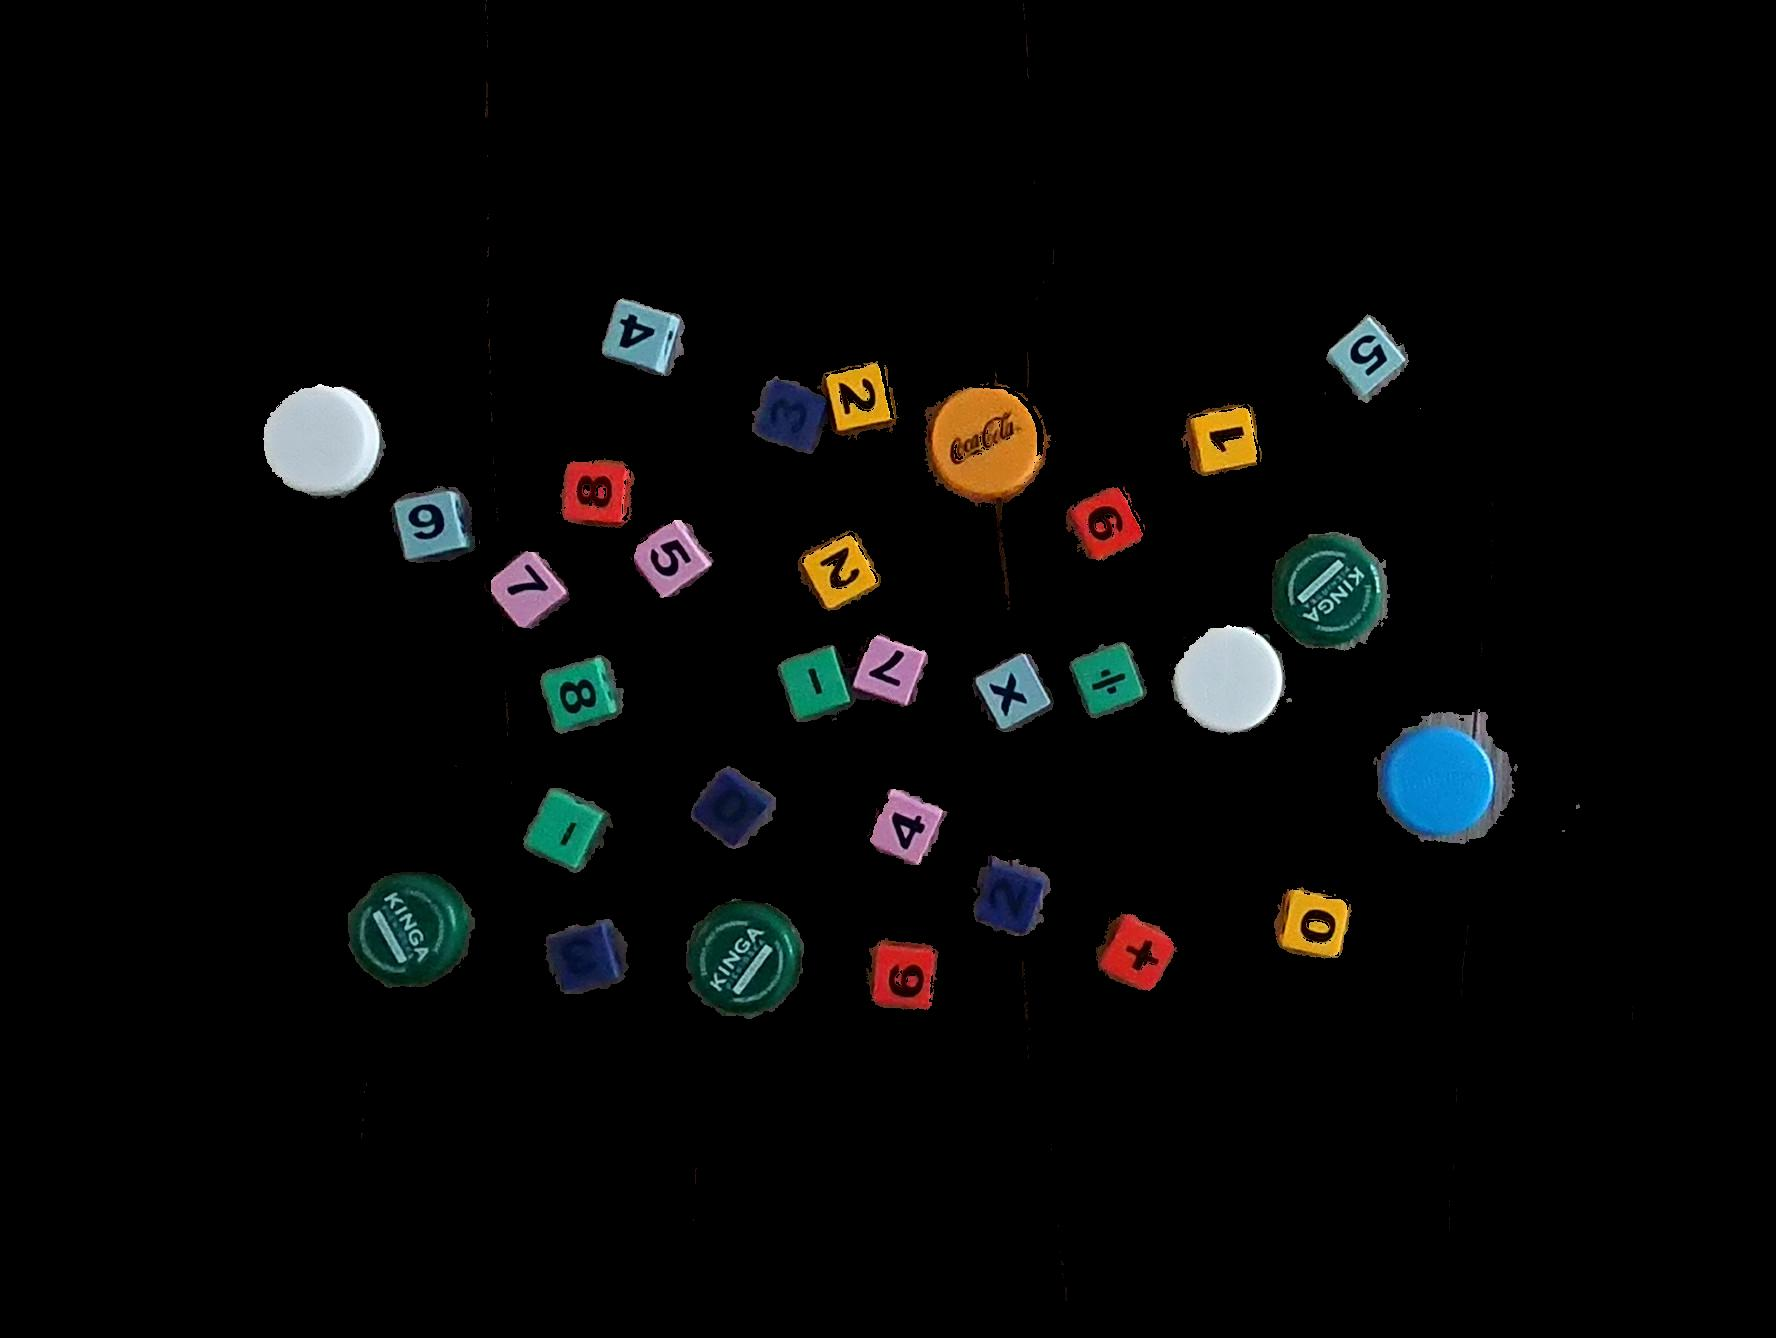
\includegraphics[scale=0.25]{img/first.jpg}
    \caption{Pierwsza pr�ba segmentacji obrazu}
    \label{good_filter}
\end{figure}

\vskip 1cm
\begin{figure}[H]
    \centering
    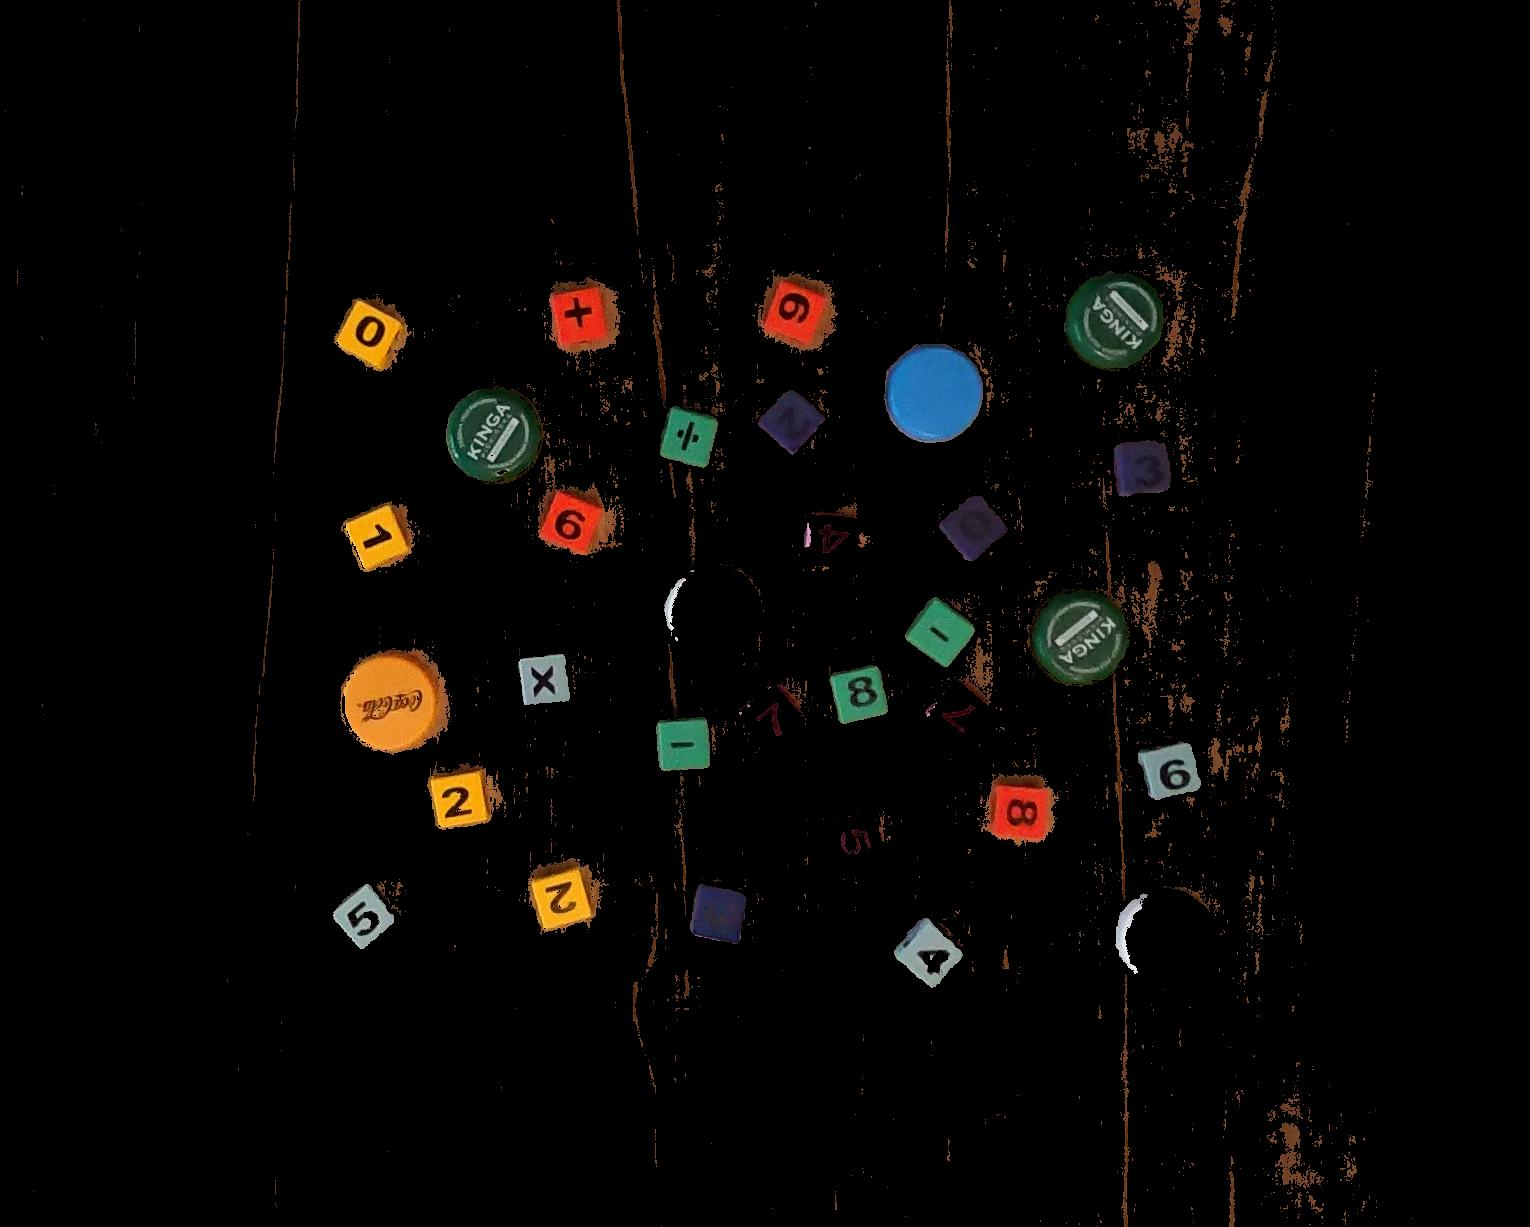
\includegraphics[scale=0.2]{img/second.jpg}
    \caption{Nieudana pr�ba segmentacji kolejnego z~obraz�w}
    \label{bad_filter}
\end{figure}

Po pr�bach odnnalezienia w�a�ciwych nastaw w~innych przestrzeniach barw zdecydowali�my si� wreszcie na skonstruowanie oddzielnego filtra dla wszystkich kolor�w znajduj�cych si� na obrazach. Na bazie wspomnianej ju� apllikacji stworzonych zosta�o 8 filtr�w maskuj�cych. Ka�dy z~nich zosta� skalibrowany r�cznie tak, aby przepuszcza� jedynie okre�lon� barw� ze wszystki trzech zdj��. Podej�cie takie, chocia� bardziej czasoch�onne, pozwala na poszerzenie marginesu b��du w~przypadku, gdy segmentowane maj� by� zdj�cia niedost�pne na etapie projektowania. Dodatkowo, aby m�c sobie pozwoli� na szersze pasma, ka�da ze stworzonych masek zosta�a przetworzona prez dedykowan� sekwencj� operacji morfologicznych. Pozwoli�y one na 'zalepienie' dziur w~masce oraz doszlifowanie kontur�w obiekt�w. Rezultaty zosta�y przedstawione na poni�szych rysunkach. Dodatkowo, do��czone zosta�o zdj�cie z~nast�pnego projektu aby pokaza�, jak filtr radzi sobie z~obrazami, pod k�tem kt�rych nie by� przygotowywany.

\begin{figure}
    \centering
    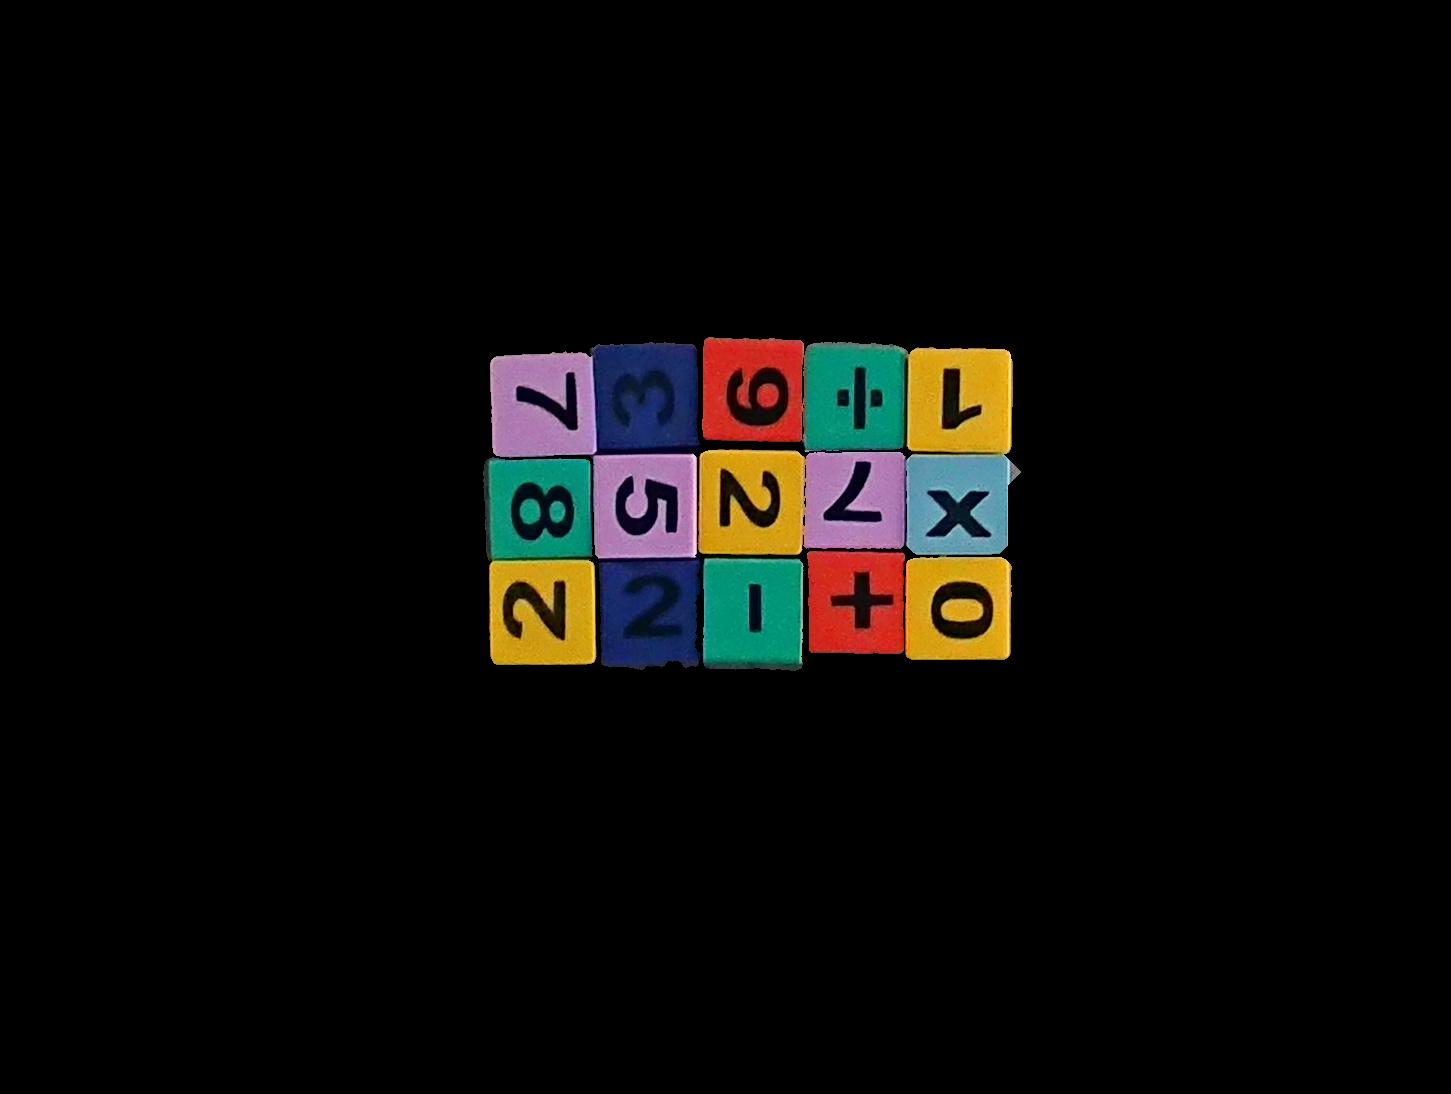
\includegraphics[scale=0.2]{img/ex_3.jpg}
    \label{ex_3}
\end{figure}

\begin{figure}
    \centering
    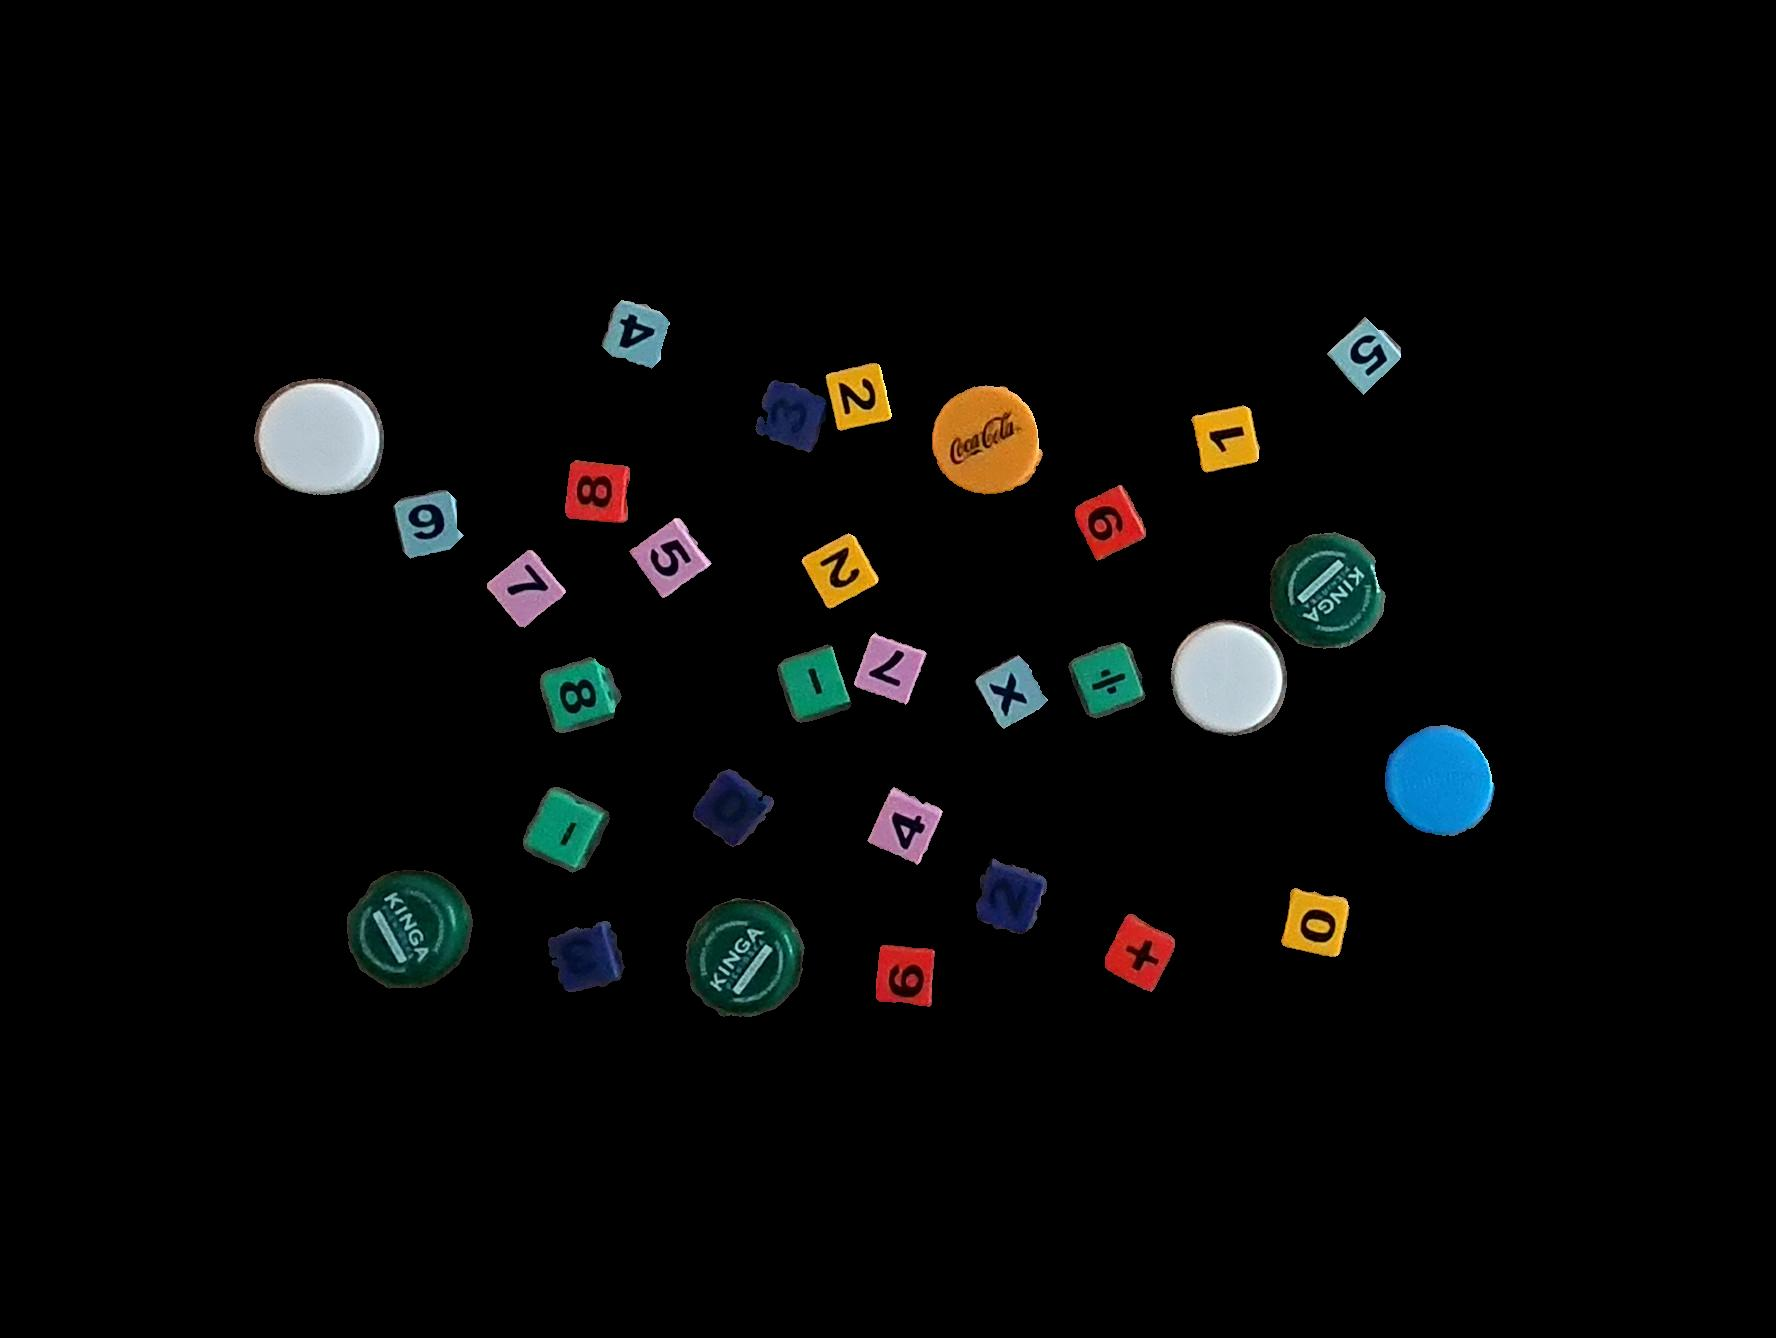
\includegraphics[scale=0.215]{img/ex_1.jpg}
    \label{ex_1}
\end{figure}

\begin{figure}
    \centering
    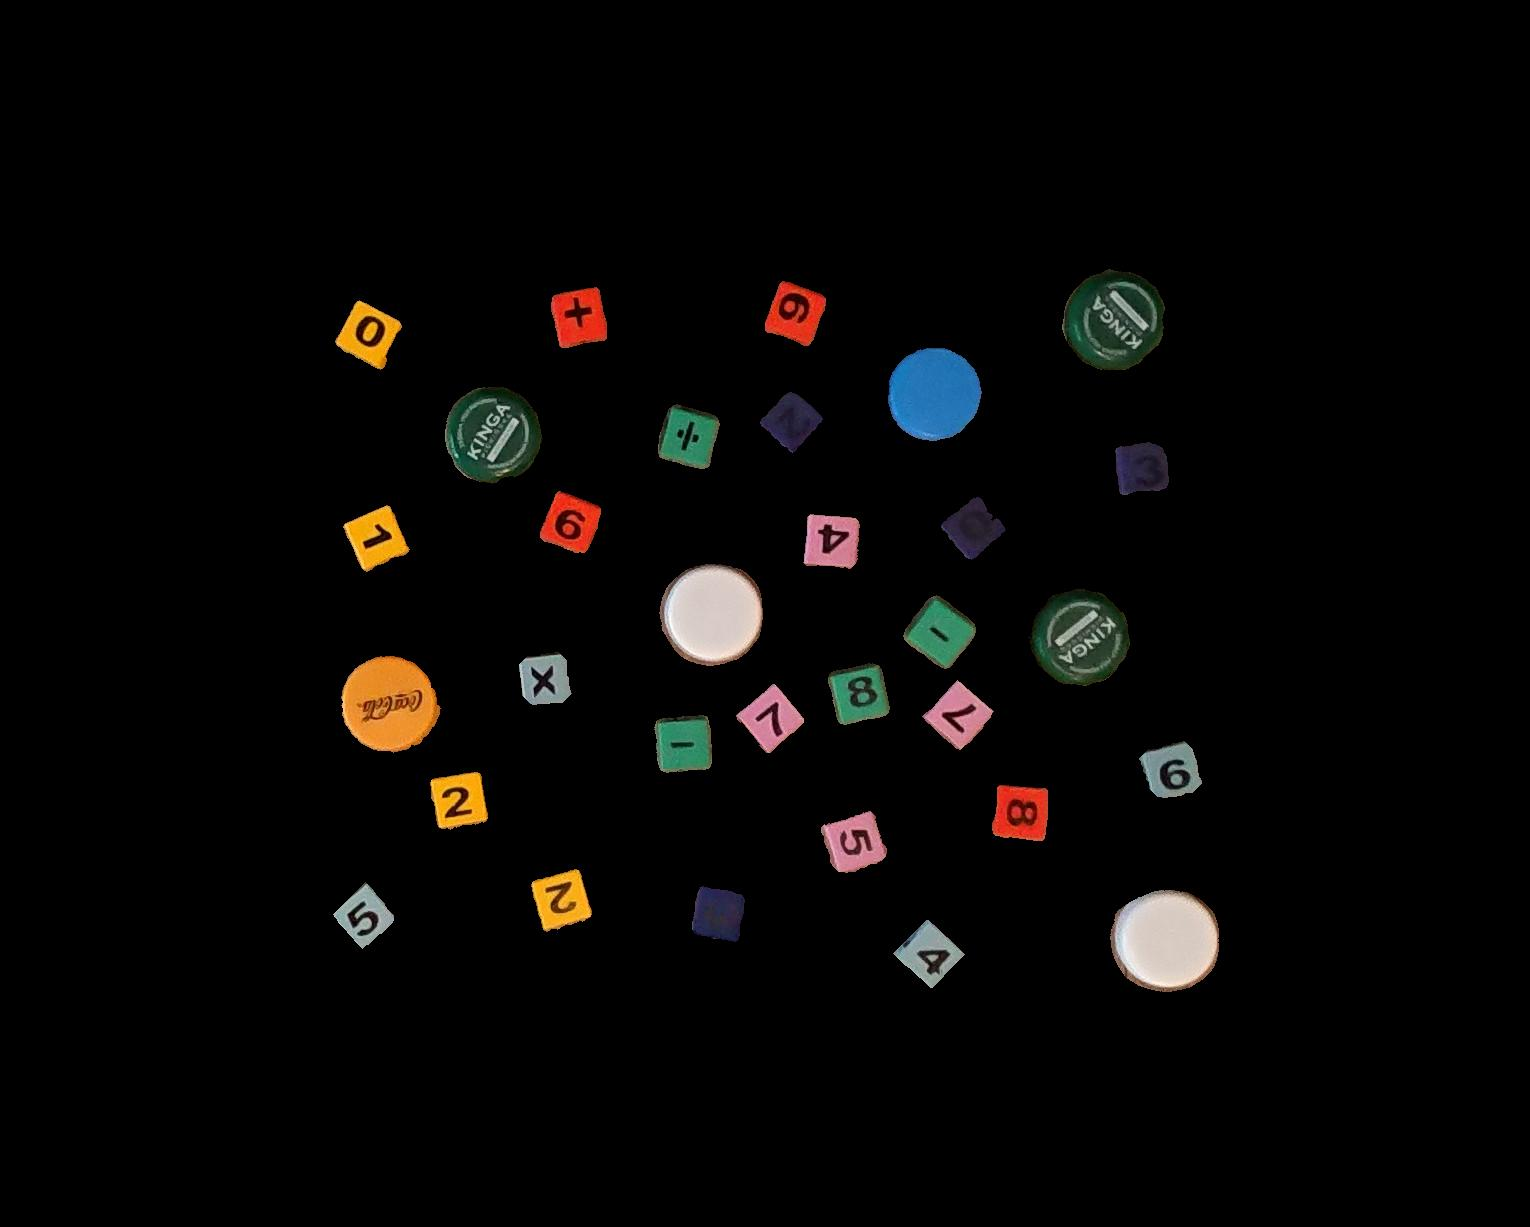
\includegraphics[scale=0.25]{img/ex_2.jpg}
    \label{ex_2}
\end{figure}

\begin{figure}
    \centering
    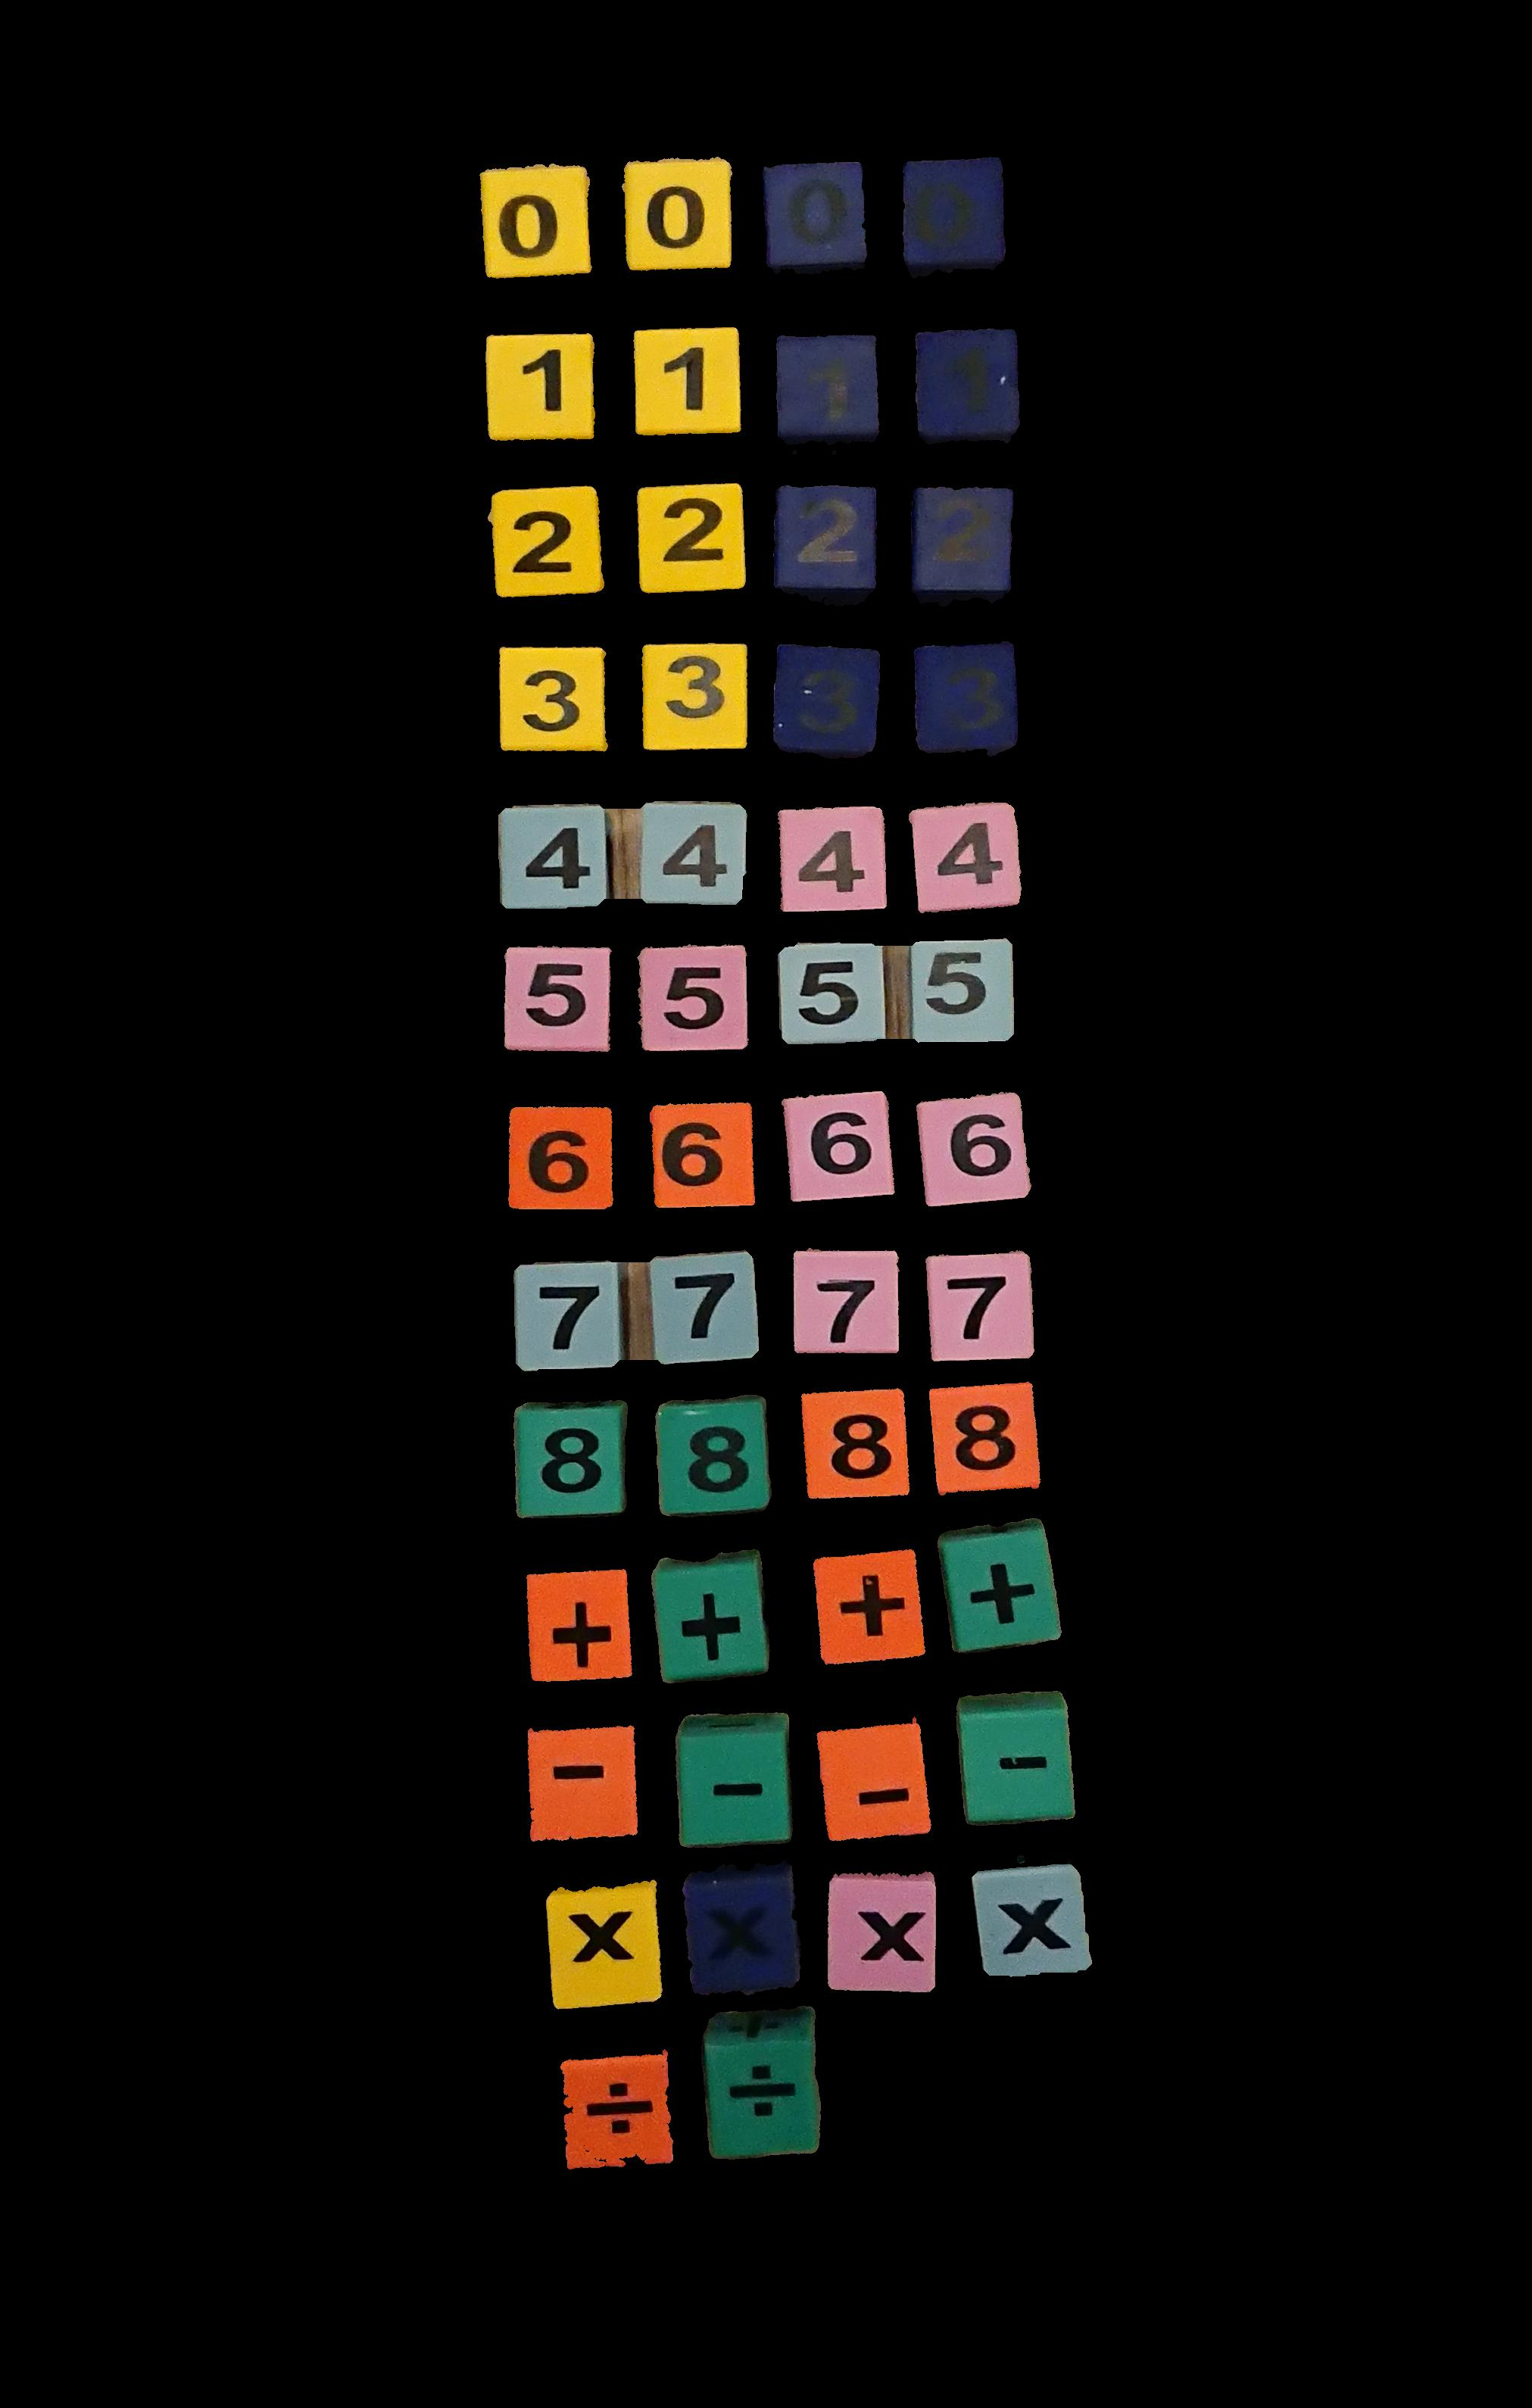
\includegraphics[scale=0.18]{img/ex_4.jpg}
    \label{ex_4}
\end{figure}




\chapter*{Analiza region�w}

Drugie zadanie, korzystaj�c z~efekt�w poprzedniego, polega�o na przeanalizowaniu przefiltrowanych zdj�� pod k�tem: kszta�tu, barwy, �rodka masy obiekt�w, orientacji obiekt�w oraz ich rozmiaru. Wszystkie te cechy mo�liwe by�y do okre�lenia dzi�ki wykorzystaniu funkcji  \verb regionprops.  Przy jej u�yciu uzyskiwali�my informacje o~po�o�eniu obiekt�w, ich powierzchni, obwodzie, punktach ekstremalnych (najbardziej wysuni�tych w~danym kierunku) oraz o~minimalnym prostok�cie opisanym na obiekcie. Dlak ka�dego rekordu zwr�conego przez funkcj� przeprowadzana by�a ta sama procedura identyfikacyjna.

W~pierwszej kolejnosci zapisywali�my do przygotowanej struktury danych po�o�enie obiektu, poniewa� warto�� ta by�a dostepna bezpo�rednio. Nast�pnie wycinany by� fragment obrazu zawieraj�cy jedynie analizowany obiekt (wykorzystano tu wspomniany wy�ej minimalny prostok�t). W~regionie tym, przekonwertowanym z~przestrzeni RGB do HSV, sprawdzana by�a najpierw najcz�ciej wystepuj�ca warto�� saturacji, a~nastepnie najcz�ciej wystepuj�ca barwa. Je�eli nasycenie przekracza�o pewien pr�g, obiekt by� klasyfikowany jako bia�y. W~pozosta�ych przypadkach kolor by� oceniany na bazie drugiego z~parametr�w.Ka�dy obiekt zosta� zaklasyfikowany do jednej z~7~gr�b kolorystycznych.

Kolejnym krokiem by�o policzenie zwarto�ci obiektu (pos�uguj�c si� warto�ciami pola i~obwodu obiektu). Jako, �e mieli�my wykryuwa� tylko 3~rodzaje kszta�t�w (kwadratowy, okr�g�y i~pozosta�e) progowanie tej warto�ci by�o wystarczaj�ce do okreslenia prawid�owego kszta�tu wi�kszo�ci obiekt�w. Gdy okre�lony zosta� kszta�t, na bazie odpowiednich wzor�w, mo�liwa by�a estymacja rozmiaru (�rednicy w~przypadku k� i~d�ugo�ci boku w~przypadku kwadrat�w). Orientacja obiekt�w zosta�a z~kolei okre�lona jako wektor zaczepiony w~�rodku masy obiektu i~skierowany w~stron� skrajnego prawego, g�rnego piksela obiektu (w~wi�kszo�ci przypadk� pozwala�o to wskaza� jeden z~rog�w obiekt�w kwadratowych). Niestety orientacja ta nie uwzgl�dnia�a orientacji znak�w znajdujacych si� na obiektach. Ich analiza by�aby zbyt z�o�ona jak na ramy tych zaj�� laboratoryjnych.

\vskip 0.8cm
\begin{figure}[H]
    \centering
    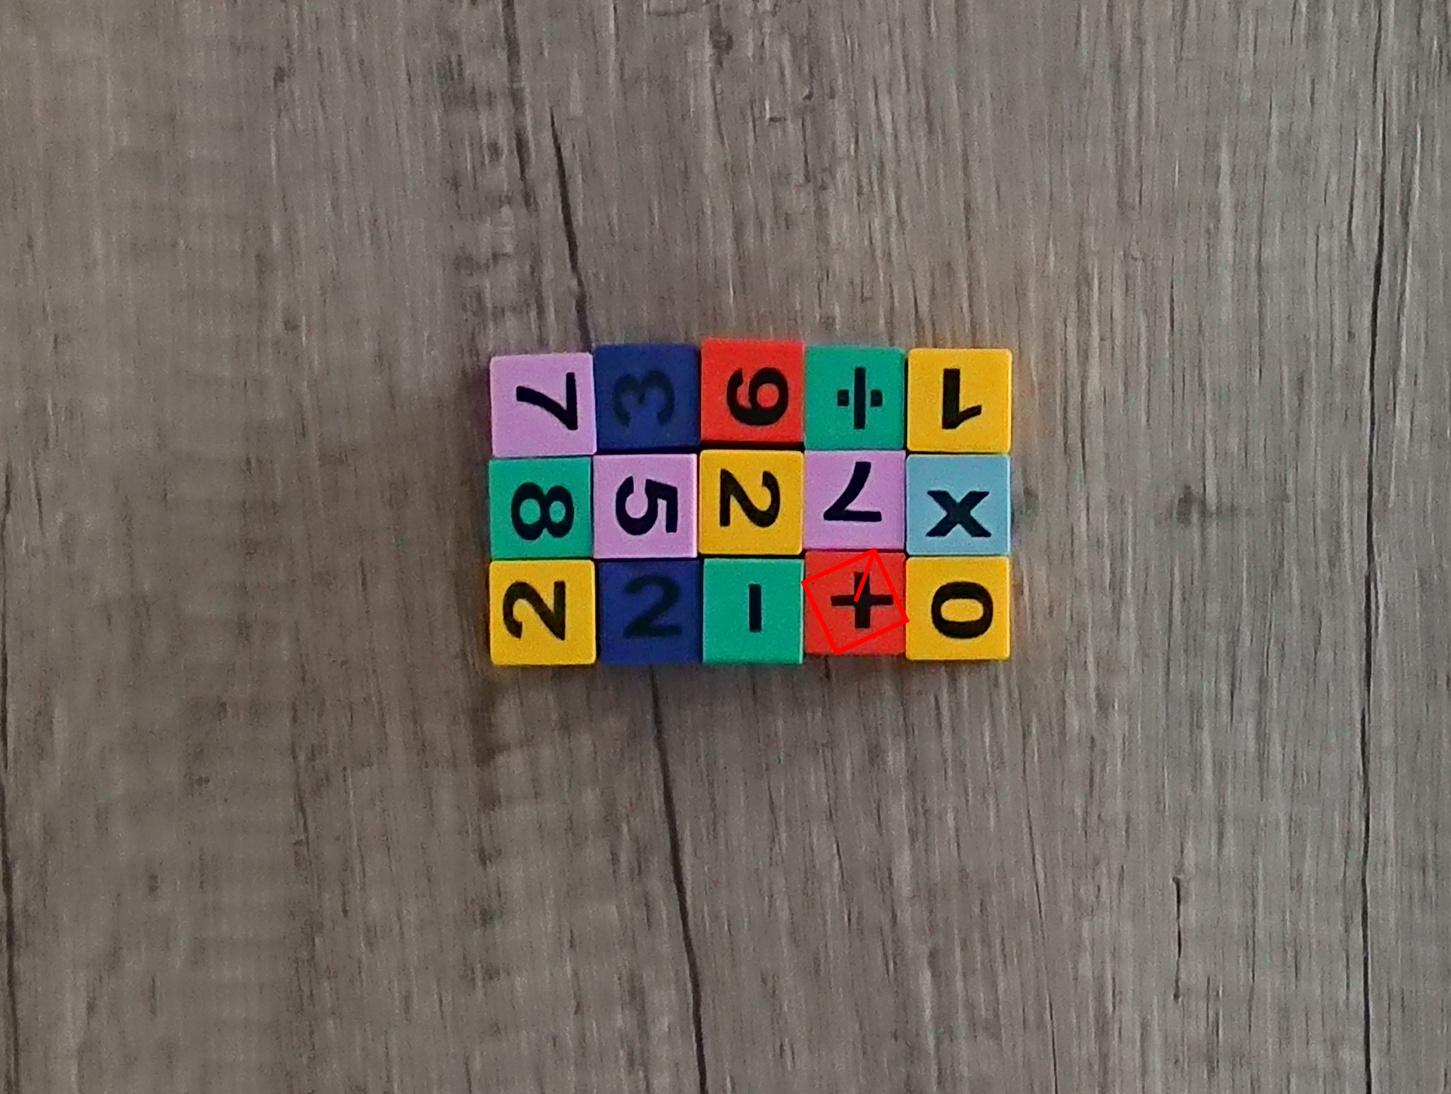
\includegraphics[scale=0.18]{img/desc_3.jpg}
    \label{ex_3}
\end{figure}
\vskip 0.8cm

Ostatecznie, na zadany obraz by�a maska, kt�ra w~spos�b wizualny ukayzwa�a efekt dzia�ania detektora - wok� ka�dego obiektu narysowany zosta� kontur o~kolorze, kszta�cie i~rozmiarze odpowiadaj�cym warto�ciom ustalonym w~trakcie analizy. Efekty naszej pracy zosta�y ukazane na zdj�ciach.

\begin{figure}
    \centering
    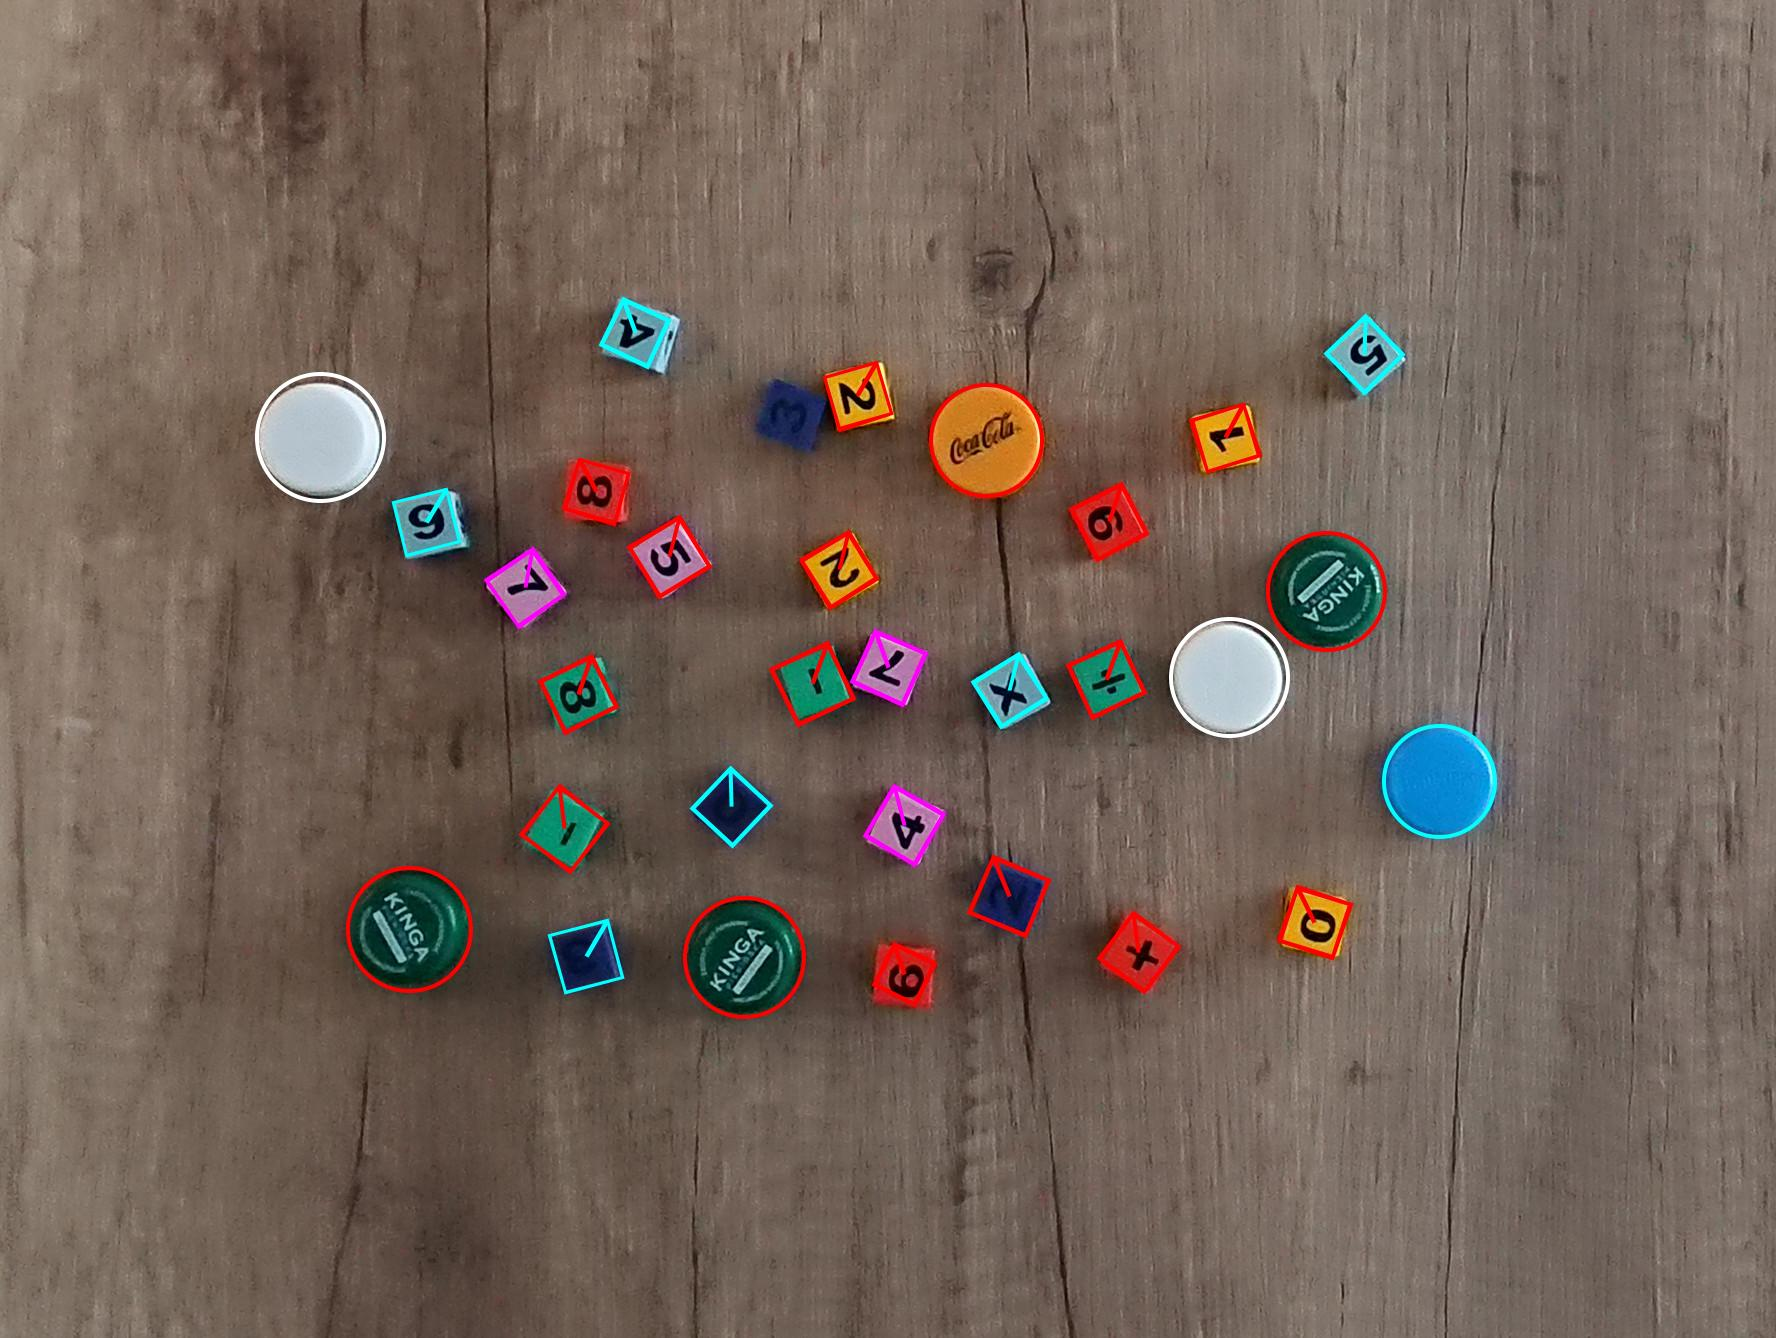
\includegraphics[scale=0.215]{img/desc_1.jpg}
    \label{ex_1}
\end{figure}

\begin{figure}
    \centering
    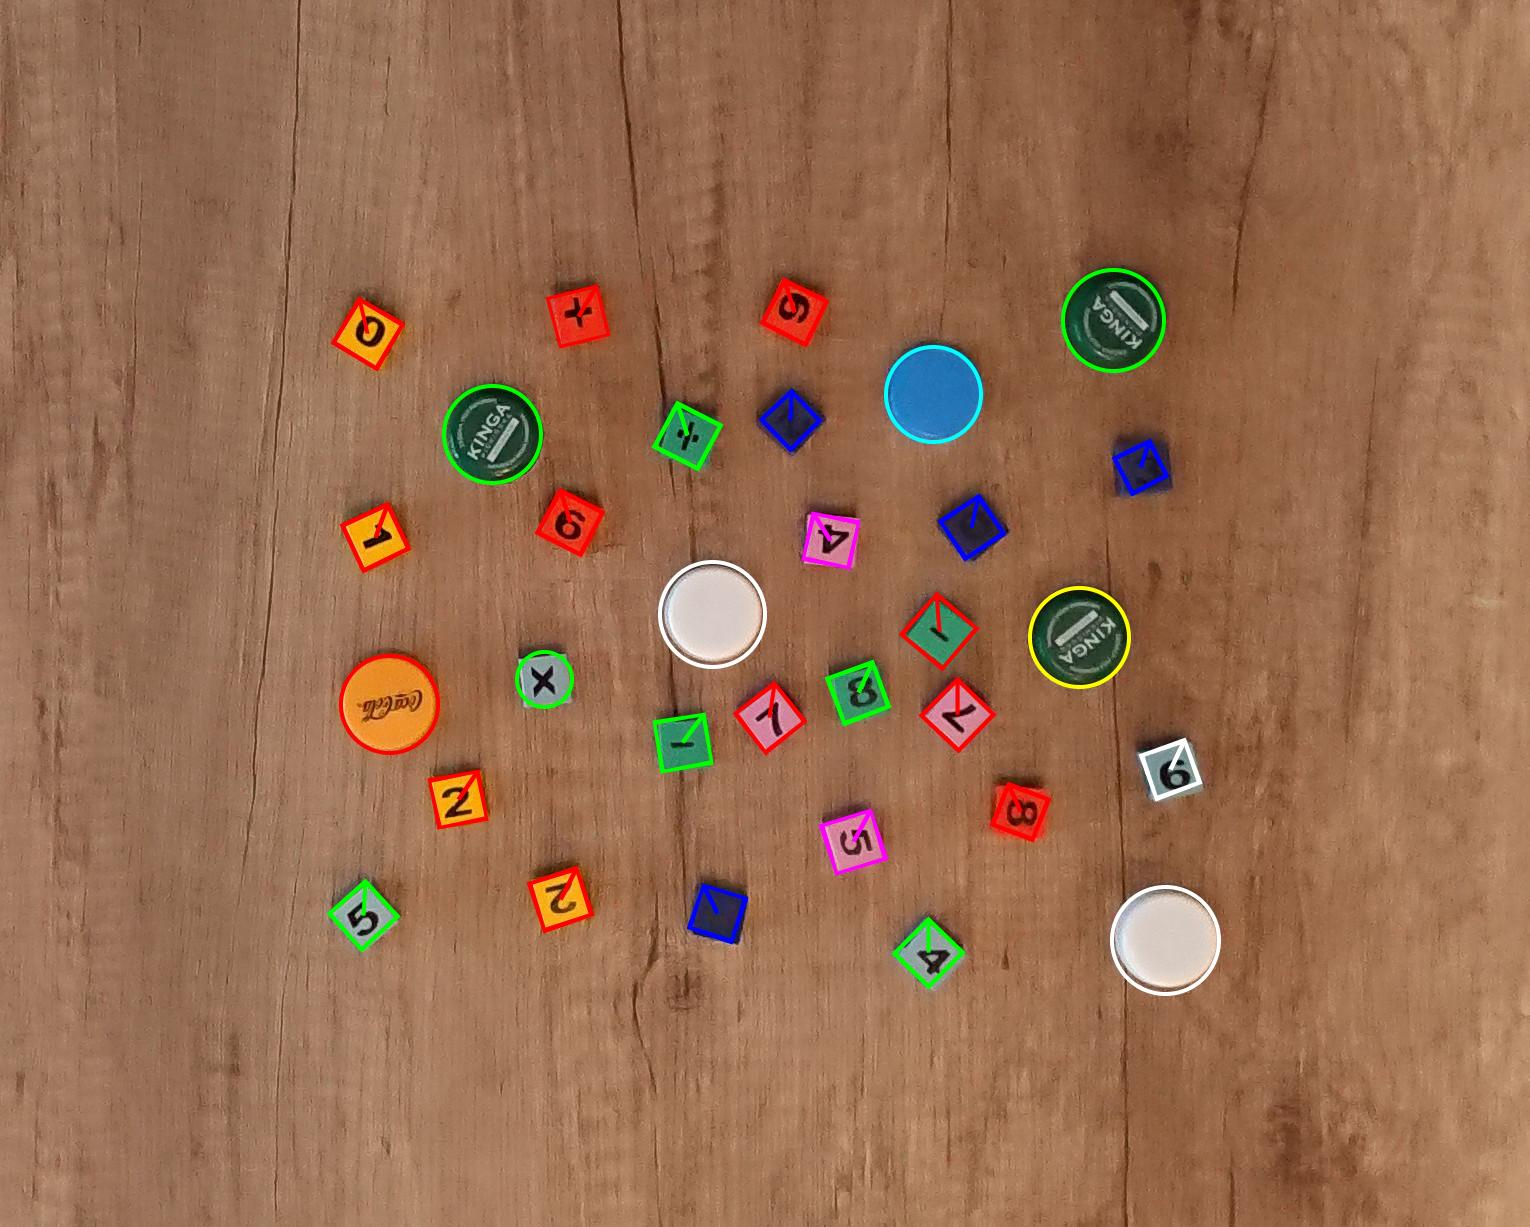
\includegraphics[scale=0.25]{img/desc_2.jpg}
    \label{ex_2}
\end{figure}

\begin{figure}
    \centering
    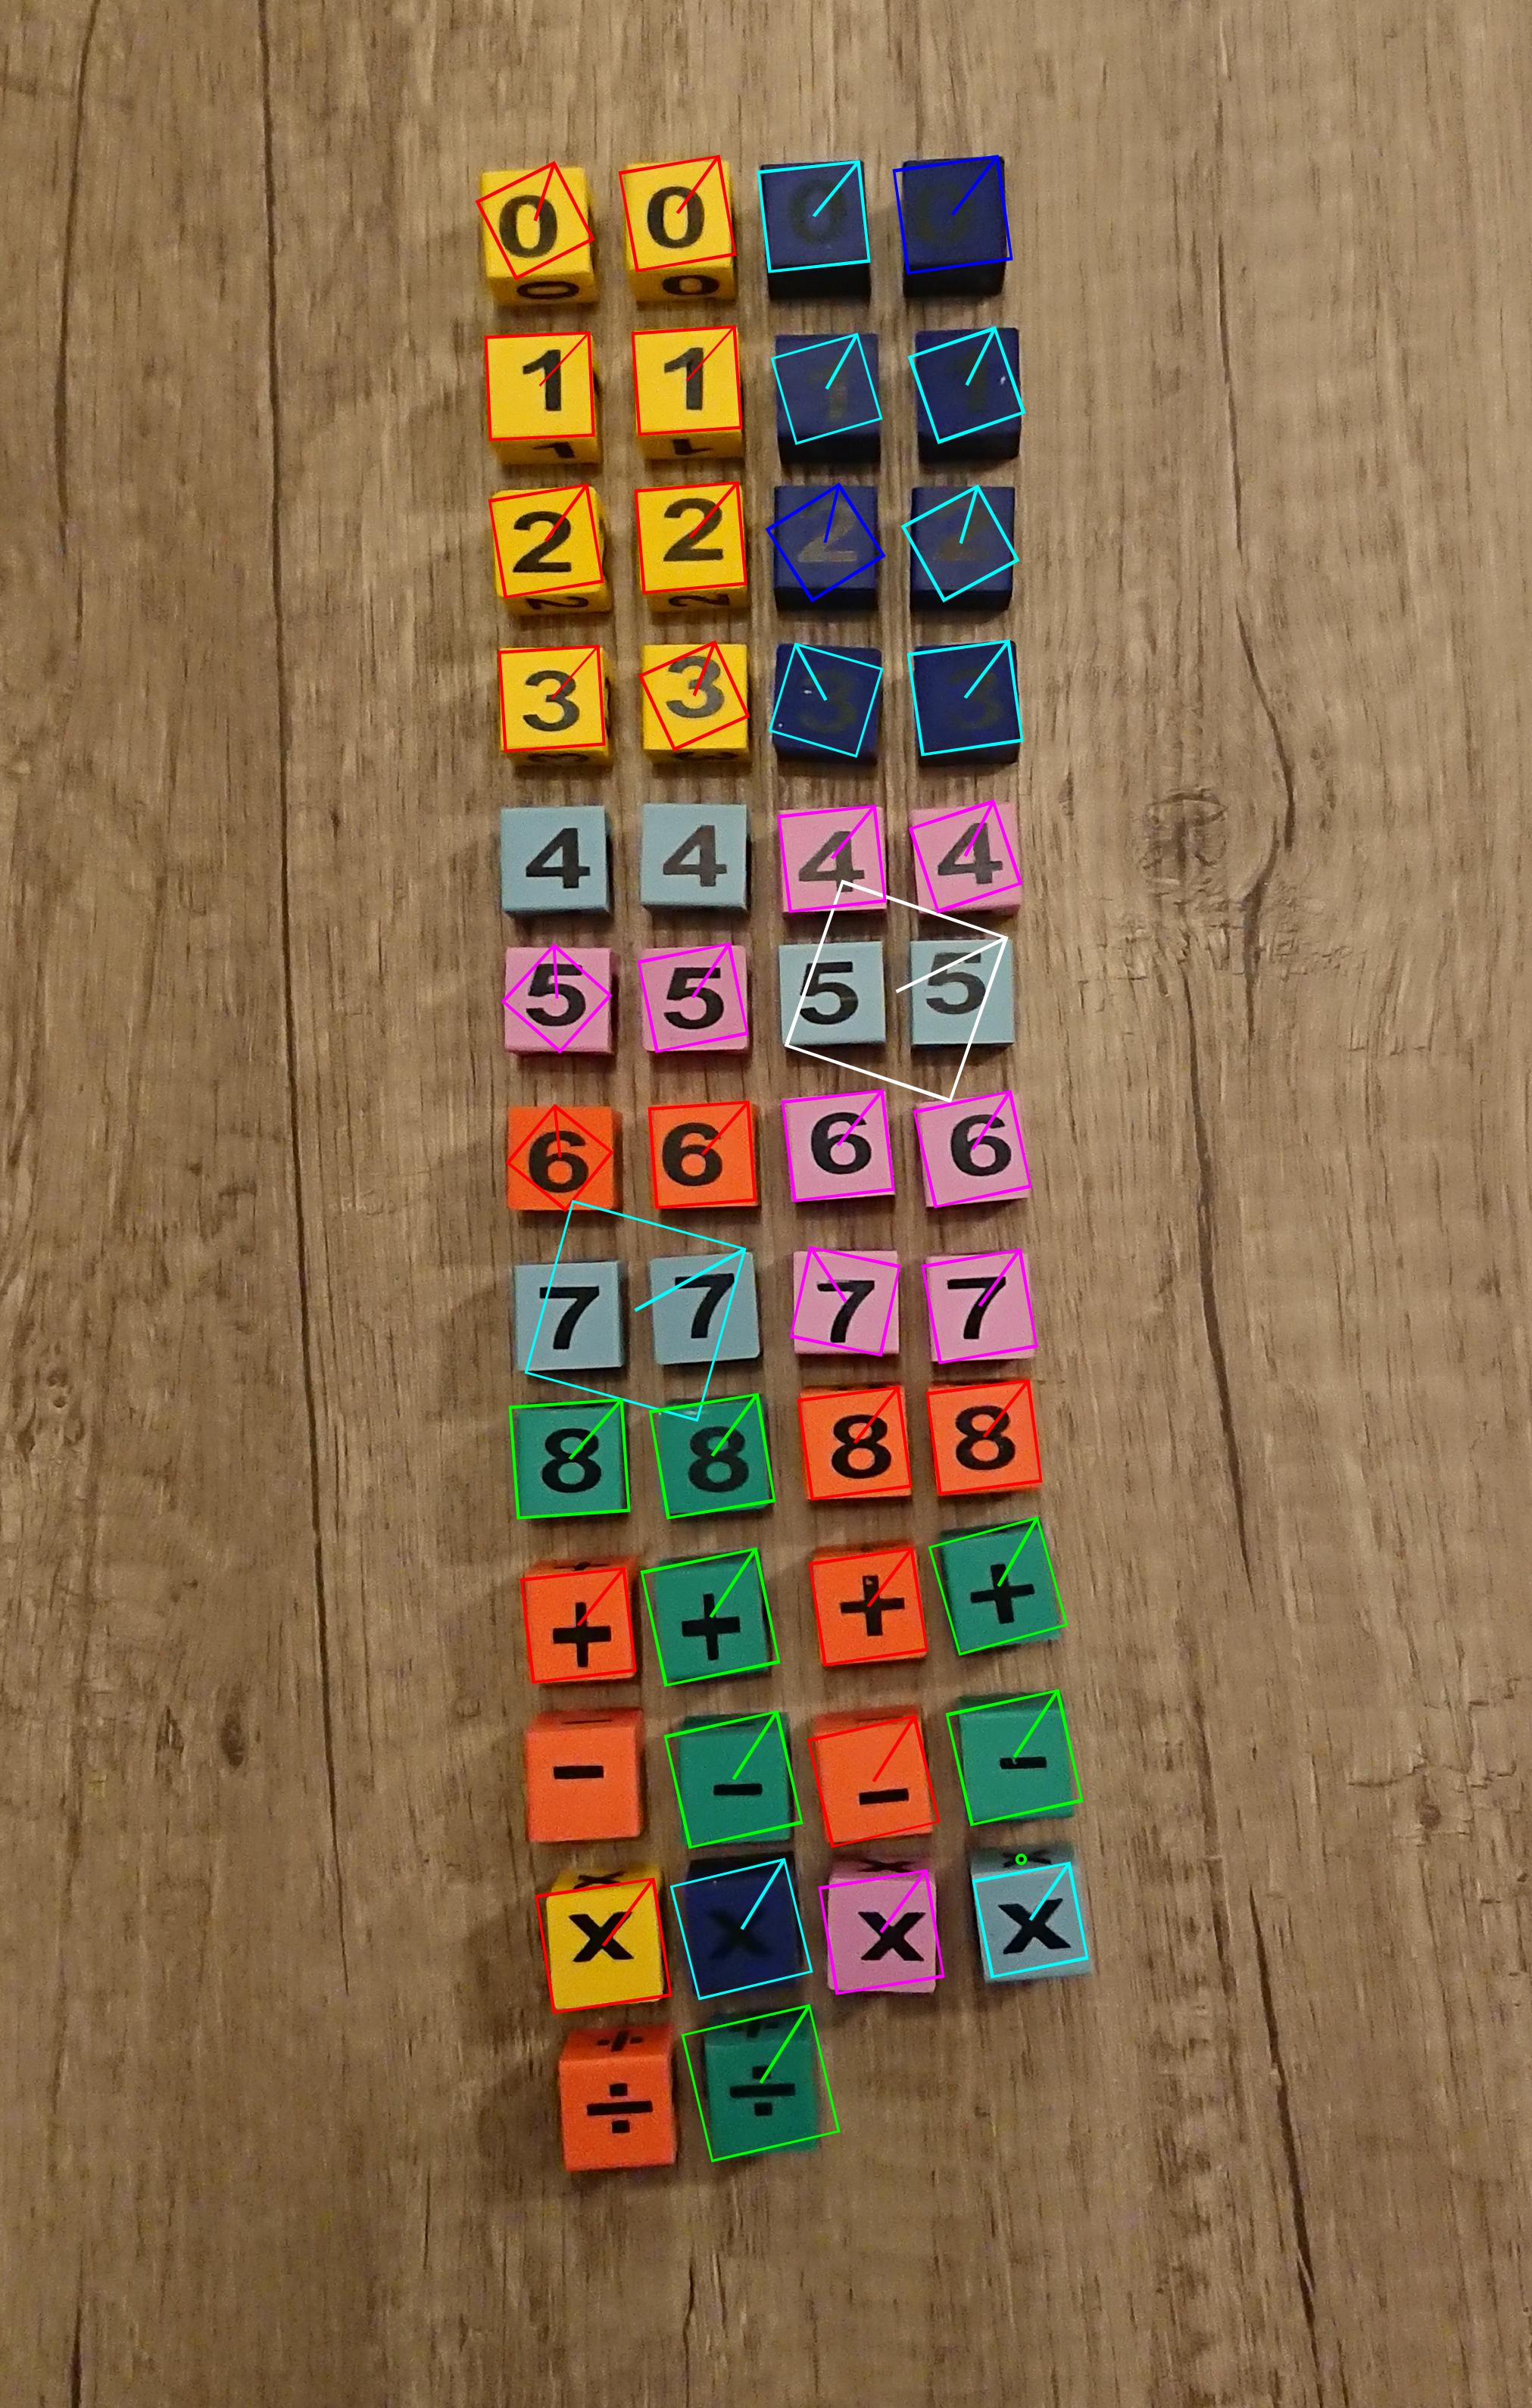
\includegraphics[scale=0.18]{img/desc_4.jpg}
    \label{ex_4}
\end{figure}


\end{document}